\section{Specific Requirements}

\subsection{External Interfaces}

\subsubsection{System Interfaces}

\paragraph{Municipality Data Exchange}

\clearpage

\paragraph{Geographic Information System} The definition of the external GIS interface is GIS dependant and will be described in a functionality-based way. The system is required to perform the following functions:

	\begin{itemize}
		\item load and filter data based on the user requested criteria
		\item cache retrieved data for the most common user requested criteria
		\item communicate the loaded and filtered data to the external GIS with the final goal of presenting the requested map to the user via the \hyperref[sec:3userinterface]{user interfaces}
	\end{itemize}
	
	The system via the external GIS is required to be capable of handling the following data visualisations:
	
	\begin{itemize}
		\item visualise the spatial location of stored violations inside a specific geographic area requested by the user
		\item visualise the spatial location of stored violations inside a specific geographic area and a specific time range requested by the user
		\item visualise the distinction between possible safe and unsafe areas identified by the system
		\item map quantities and concentrations, such as where the most and least number of violations occurred, highlighting the streets (and areas) with the highest frequency of violations
		\item map the change of quantities and concentrations inside a specific geographic area and a specific time range requested by the user
	\end{itemize}

	\begin{figure}[h]
		\centering
		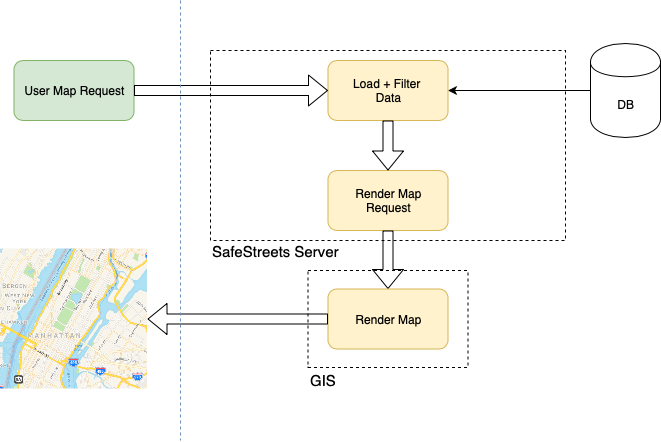
\includegraphics[width=320pt]{diagrams/GIS.png}
		\caption{
			\label{fig:externalGIS} GIS Interaction Diagram}
	\end{figure}

\subsubsection{User Interfaces}
\label{sec:3userinterface}

\subsubsection{Hardware Interfaces}
\subsubsection{Software Interfaces}
\subsubsection{Communication Interfaces}


\subsection{Functional Requirements}
Definition of use case diagrams, use cases and associated sequence/activity diagrams, and mapping on requirements

\subsection{Performance Requirements}

\subsection{Logical Database Requirements}

\subsection{Design Constraints}

\subsubsection{Standards Compliance}
\subsubsection{Hardware Limitations}
\subsubsection{Other?}

\subsection{Software System Attributes}

\subsubsection{Reliability}
\subsubsection{Availability}
\subsubsection{Security}
\subsubsection{Maintainability}
\subsubsection{Portability}





\subsection{Functional Requirements}
The following requirements are derived in order to achieve the specified goals.
\subsubsection{Goals}
	\begin{description}
		\item \ref{goal:register}\ Allow guest users to register to the system
			\begin{enumerate}[label=\textbf{R\arabic*}]
			
  				\item The system must require the \emph{guest} user to insert his fiscal code, a username, a valid e-mail and a password to identify him
  				
   				\item The system must check that the validity of the data inserted by the \emph{guest} user namely avoid duplicates, invalid fiscal codes and too weak passwords
   				
   				\item The system must send an e-mail to the \emph{guest} user to verify the e-mail address given during the registration
   
  			\end{enumerate}
  				
				\textbf{DA2} Internet connection always works correctly
				
				\textbf{DA6} The smartphone of the user runs iOS (9 or later) or Android (Jelly Bean or later)
			
  			
		\item \ref{goal:login}\ Allow registered users to authenticate to the system
			\begin{enumerate}[label=\textbf{R\arabic*}, resume]
  				\item The system must require the user to insert his username and password to authenticate to the system
   				\item The system must be able to check if the username and password pair correspond to a user correctly registered to the system and grant the access to that user

			\end{enumerate}
			
			\textbf{DA2} Internet connection always works correctly
			
			\textbf{DA5} The DBMS always works properly so that the information in the DB are always accessible
			
		\item \ref{goal:userTransfer}}\ Allow users to transfer data to the system describing occurred violations, including the suitable metadata to describe the submitted violation			\begin{enumerate}[resume*]
				\item The system must allow the user to take a picture of the violation and the plate from the mobile application
  				\item The system must allow the user to manually insert the license plate number in order to help the recognition algorithm
  				\item The system must be able to retrieve the license plate of the vehicle running an algorithm to recognise it
  				\item The system must be able to verify that the license plate number is valid and registered to a vehicle
  				\item The system must require the user to specify the type of violation
  				\item The system must allow the user to provide the location of the violation, manually specifying the address, picking it up from the map or using the GPS of the device
   			\end{enumerate}
   			
   			\textbf{C2} The quality of the picture is sufficient to recognise the plate number (min resolution 320x240)
   			
			\textbf{C3} Internet connection must be strong enough to allow the upload of the picture in a reasonable amount of time (supported technologies are 3G, 4G and 5G due to the performance requirement)
			
			\textbf{DA1} GPS position of all users is always obtainable
			
			\textbf{DA2} Internet connection always works correctly
			
		\item \ref{goal:avoidLeaks}}\ Ensure that the chain of custody of the information provided by the users is never broken, and the information is never altered or manipulated			\begin{enumerate}[resume*]
   				\item The system must provide a secure channel to communicate with the users
   				\item The system must encrypt the connection with the users in order to protect the process of providing data
   				\item The system must adopt security measures to prevent malicious accesses and to protect sensible data
   				\item Questo davvero non lo so mori miei
  			\end{enumerate}
  			
  			
		
		\item \ref{goal:municipalityTransfer}}\ Allow the system to retrieve data about the accidents that occur on the territory and data about issued tickets via the municipality provided service
			\begin{enumerate}[resume*]
   				\item The system must be able to retrieve data about accidents from municipality systems 
   				\item The system must be able to process data retrieved from municipality
   				\item The system must be able to elaborate accidents and violations information to extract data about unsafe areas
   				\item The system must be able to provide data to municipality systems to suggest possible interventions to increase safety in a specific area
  			\end{enumerate}
  			
  			\textbf{DA2} Internet connection always works correctly
  			
			\textbf{DA3} Municipality services are always reachable
  			
  		\item \ref{goal:statistics}}\ Allow the system to cross the information submitted by the users and the information retrieved from the municipality to build statistics
  			\begin{enumerate}[resume*]
  				\item 
   				
  			\end{enumerate}
  		\item \ref{goal:ticketsInformation}\ Access the municipality archives of emitted tickets and build statistics based on the retrieved information
  			\begin{enumerate}[resume*] 
  				\item The system must be able to retrieve data about tickets issued by the municipality 
   				\item The system must be able to process data retrieved from municipality
   				\item The system must be able to elaborate issued tickets information to generate statistics about useful violations provided by users
   			\end{enumerate}
   	\end{description}
  	
\subsection{Performance Requirements}
	The system should ensure acceptable response times in the interactions with the user, which strictly depends on the number of concurrent users and the connection speed.
\newline
The processes of providing data and loading the map of safe and unsafe areas shouldn't be too slow.
\subsection{Software System Attributes}
	\subsubsection{Availability}
	The system must be available 99,9\% of the time (up to 8,76 hours per year of downtime). The system should be accessible 24 hours per day.
	\subsubsection{Security}
	Users personal information and payment information are encrypted and must be protected during transmission, as already stated the PTPP protocol will be used to ensure encryption through the network.
	Restricted access APIs must check that who tries to use them is actually allowed to do so.
	\subsubsection{Portability}
	The system must be also accessible by the most common mobile platforms (iOS and Android devices).

